\documentclass[a4paper]{article}
\usepackage[brazilian]{babel}
\usepackage{subfig}
\usepackage{booktabs}
\usepackage{graphicx}
%-----------------------------------------------------------------
\title{Projeto 2: Simula\c{c}\~ao de modelo presa-predador com acidente com poluente.}
\author{122830 Alcides Goldoni Junior\\
  \small MS 680 - Modelos matem\'{a}ticos aplicados a Biologia\\
  %\small Unicamp 
}%Fechando Title
\begin{document}
\maketitle
%Seções
%-----------------------------------------------------------------
\section{Introdu\c{c}\~{a}o}
\\
\\
Nesse projeto irei simular a preda\c{c}\~ao de tr\^es esp\'ecies por um predador que se alimenta exclusivamente dessas esp\'ecies.
\\
\\
Em um determinado instante no tempo, ser\'a introduzido no meio, um acidente com poluente, onde ele \'e despejado de uma s\'o vez e sua concentra\c{c}\~ao decai ao longo do tempo. Esse poluente afeta apenas as esp\'ecies predadas.
\\
\\
Vou analisar o comportamento das esp\'ecies antes e depois do acidente, verificando se existe estabilidade na conviv\^encia ou se elas chegar\~ao a se extinguir.
\\
\\
\section{Modelagem}
Tr\^es esp\'ecies vivem em um lago suficientemente grande. Essas esp\'ecies competem pelos recursos do meio ambiente mas n\~ao se predam. Nesse mesmo lago, existe uma quarta esp\'ecie que predadora das outras tr\^es.
\\
\\
Um acidente ocorre e despeja um certa quantidade de poluente nesse lago, afetando negativamente as esp\'ecies que s\~ao predadas mas n\~ao afetando a predadora. A concetra\c{c}\~ao do poluente sofre um decaimento ao longo do tempo de forma muito lenta, afetando outras gera\c{c}\~oes da popula\c{c}\~ao de presas.
\\
\\
Partindo das premissas acima, vou modelar a equa\c{c}\~ao que descreve a situa\c{c}\~ao utilizando o modelo de crescimento populacional descrito por Verhulst e um decaimento constante para o poluente.
\\\
\\
Dessa forma, o sistema de equa\c{c}\~oes abaixo modela o problema:
\\
\\
\begin{equation}
\left\{\begin{array}{l}
\frac{\delta A}{\delta t} =  \lambda_A (A + B + C + D)(2 - \frac{A + B + C +D}{K}) -\alpha_1AD - \alpha_2PA  \\
\\
\frac{\delta B}{\delta t} =  \lambda_B (A + B + C + D)(1 - \frac{A + B + C +D}{K}) -\beta_1BD - \beta_2BA  \\
\\
\frac{\delta C}{\delta t} =  \lambda_C (A + B + C + D)(1 - \frac{A + B + C +D}{K}) -\gamma_1CD - \gamma_2CA  \\
\\
%\frac{\delta D}{\delta t} =  \lambda_D (A + B + C + D)(1 - \frac{A + B + C +D}{K}) + \alpha_1AD + \beta_1 BD + \gamma_1CD  \\
\frac{\delta D}{\delta t} =  \lambda_D (A + B + C + D)(1 - \frac{A + B + C +D}{K}) + \mu_1AD + \mu_2 BD + \mu_3CD  \\
\\
\frac{\delta P}{\delta t} = - \varepsilon P \\
\end{array}
\end{equation}
\\
\\
Onde:
\\
\\
$A, B$ e $C$ s\~ao as esp\'ecies predadas;
\\
\\
$D$ \'e a esp\'ecie predadora;
\\
\\
$P$ \'e o poluente;
\\
\\
$\lambda$ \'e a taxa de crescimento de cada popula\c{c}\~ao;
\\
\\
$\alpha_1$ \'e a taxa de decrescimento da popula\c{c}\~ao $A$ por preda\c{c}\~ao;
\\
\\
$\alpha_2$ \'e a taxa de decrescimento da popula\c{c}\~ao $A$ por polui\c{c}\~ao;
\\
\\
$\beta_1$ \'e a taxa de decrescimento da popula\c{c}\~ao $B$ por preda\c{c}\~ao;
\\
\\
$\beta_2$ \'e a taxa de decrescimento da popula\c{c}\~ao $B$ por polui\c{c}\~ao;
\\
\\
$\gamma_1$ \'e a taxa de decrescimento da popula\c{c}\~ao $C$ por preda\c{c}\~ao;
\\
\\
$\gamma_2$ \'e a taxa de decrescimento da popula\c{c}\~ao $C$ por polui\c{c}\~ao;
\\
\\
$\mu$ \'e a taxa de crescimento da popula\c{c}\~ao $D$ em rela\c{c}\~ao a cada presa;
\\
\\
$\varepsilon$ \'e o decaimento da polui\c{c}\~ao.
\\
\\
\'E esperado que quando as esp\'ecies presadadas comecem a diminuir devido a polui\c{c}\~ao, o predador, em um primeiro momento, continue crescendo, mas, em seguida comece a diminuir devido a falta de alimentos.
\\
\\
J\'a as presas, \'e esperado que elas cres\c{c}am at\'e que o acidente aconte\c{c}a, ap\'os isso, \'e esperado que elas diminuam bruscamente at\'e que estabilizem.
\\
\\
N\~ao \'e esperado que nenhuma das popula\c{c}\~oes cheguem a extin\c{c}\~ao, mas dependendo do decaimento do poluente, isso pode ocorrer.
\\
\\
\section{Simula\c{c}\~oes}
Para a simula\c{c}\~ao, foi utilizado a linguagem de programa\c{c}\~ao Python e a biblioteca Matplotlib para gerar os gr\'aficos. A simula\c{c}\~ao ocorreu em um notebook Dell Latide E6510 com processador Intel(R) Core(TM) i7 CPU Q 840 @ 1.87GHz, 1TB de HD e 8GB de mem\'oria RAM.
\\
\\
Os valores iniciais da popula\c{c}\~ao das presas s\~ao significativamente maiores do que o valor inicial do predador a fim de simular que as presas s\~ao peixes bem menores que os predadores e, dessa forma, tem uma popula\c{c}\~ao maior no lago.
\\
\\
J\'a o valor inicial da polui\c{c}\~ao \'e zero, pois nessa simula\c{c}\~ao o acidente ocorre semanas depois do inicio da simula\c{c}\~ao.
\\
\\
Da mesma forma que os valores iniciais de cada popula\c{c}\~ao, a taxa de crescimento das presas \'e significativamente maior que a taxa de crescimento do predador.
\\
\\
O valor do decaimento da polui\c{c}\~ao foi escolhido de forma que a polui\c{c}\~ao permancesse no lago por tempo suficiente para que atingisse v\'arias gera\c{c}\~oes, tanto das presas quanto do predador.
\\
\\
A capacidade de suporte foi escolhida de forma aleat\'oria. Sendo apenas um n\'umero suficientemente maior que a soma dos valores iniciais.
\\
\\
Valores utilizados para a simula\c{c}\~ao:
\\
\\
\begin{table}[ht!]
\centering
\caption{Valores da simula\c{c}\~ao para as presas}
\begin{tabular}{|c|c|c|c|c|c|c|c|}
Par\^ametro & Valor & Crescimento& Valor & Decrecimento & Valor& Decrecimento & Valor\\
& & & &por Preda\c{c}\~ao & &por Polui\c{c}\~ao &\\
\hline
Esp\'ecie A & 30000 & $\lambda_A$ & 0.024  & $\alpha_1  $ & 0.00000005  & $\alpha_2 $ & 0.00054   \\
Esp\'ecie B & 20000 & $\lambda_B$ & 0.026  & $\beta_1   $ & 0.00000008  & $\beta_2  $ & 0.00056 \\
Esp\'ecie C & 10000 & $\lambda_C$ & 0.028  & $\gamma_1  $ & 0.00000009  & $\gamma_2 $ & 0.00058  \\
\end{tabular}
\end{table}
\\
\\
\begin{table}[ht!]
\centering
\caption{Valores da simula\c{c}\~ao para predadores}
\begin{tabular}{|c|c|c|c|c|c|}
Par\^ametro & Valor & Crescimento & Valor & Crecimento por preda\c{c}\~ao & Valor\\
\hline
Esp\'ecie D & 1000   & $\lambda_D$ & 0.001 & $\mu$ & 0.000000002 
\end{tabular}
\end{table}
\\
\\
Ainda existe os valores de polui\c{c}\~ao igual cem e $\varepsilon$  que \'e o decaimento com valor de 0.05.
\\
\\
Temos a capacidade de suporte $K$ com valor de 100000 indiv\'iduos.
\\
\\
N\'umero de semanas $n$ igual a 106 e a semana em quem ocorre o acidente $x$, semana 25.
\\
\\
Com esses valores, temos os seguintes gr\'aficos:
\\
\begin{figure}[!htb]
\centering
\caption{Gr\'afico de decaimento da concentra\c{c}\~ao do poluiente}
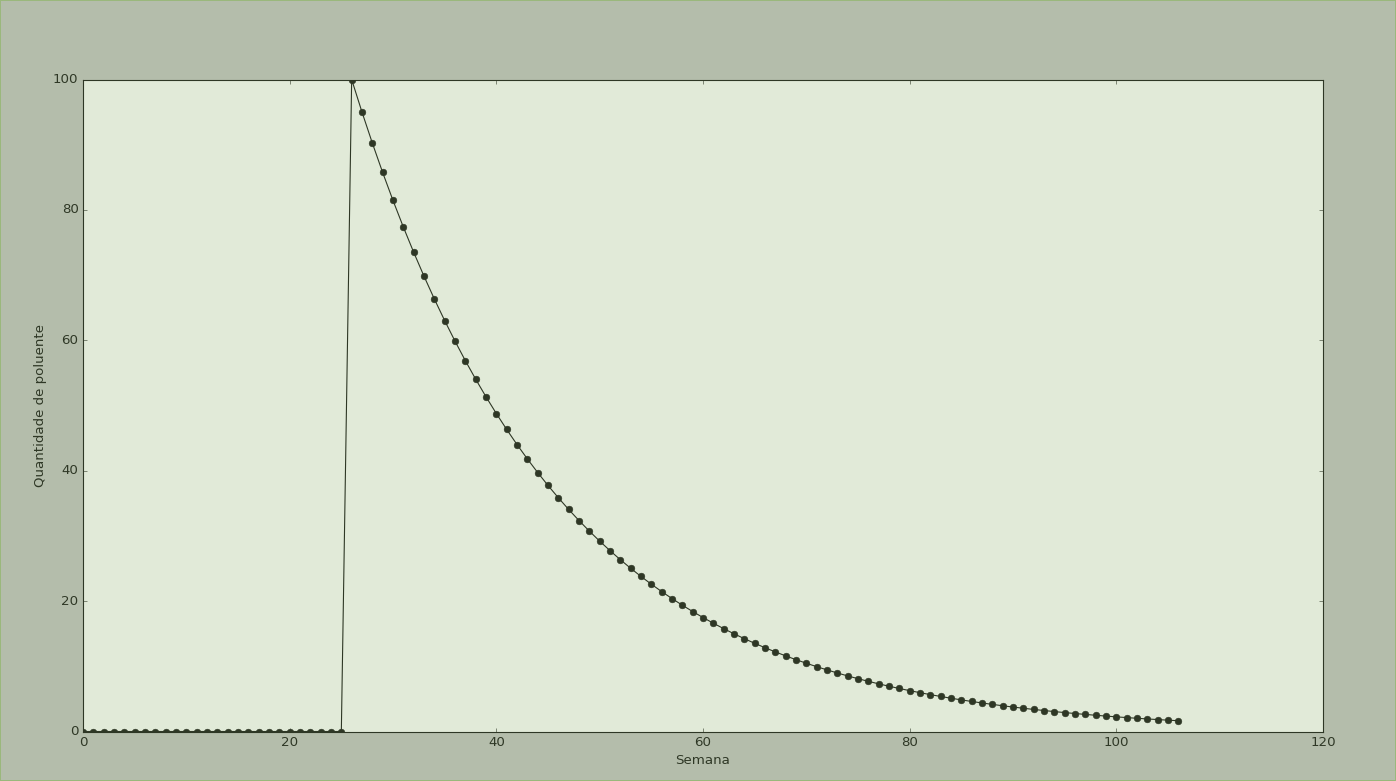
\includegraphics[scale=0.25]{graf_poluicao.png}
\end{figure}
\\
\begin{figure}[!htb]
\centering
\caption{Gr\'afico da intera\c{c}\~ao entre presa, predador e poluente}
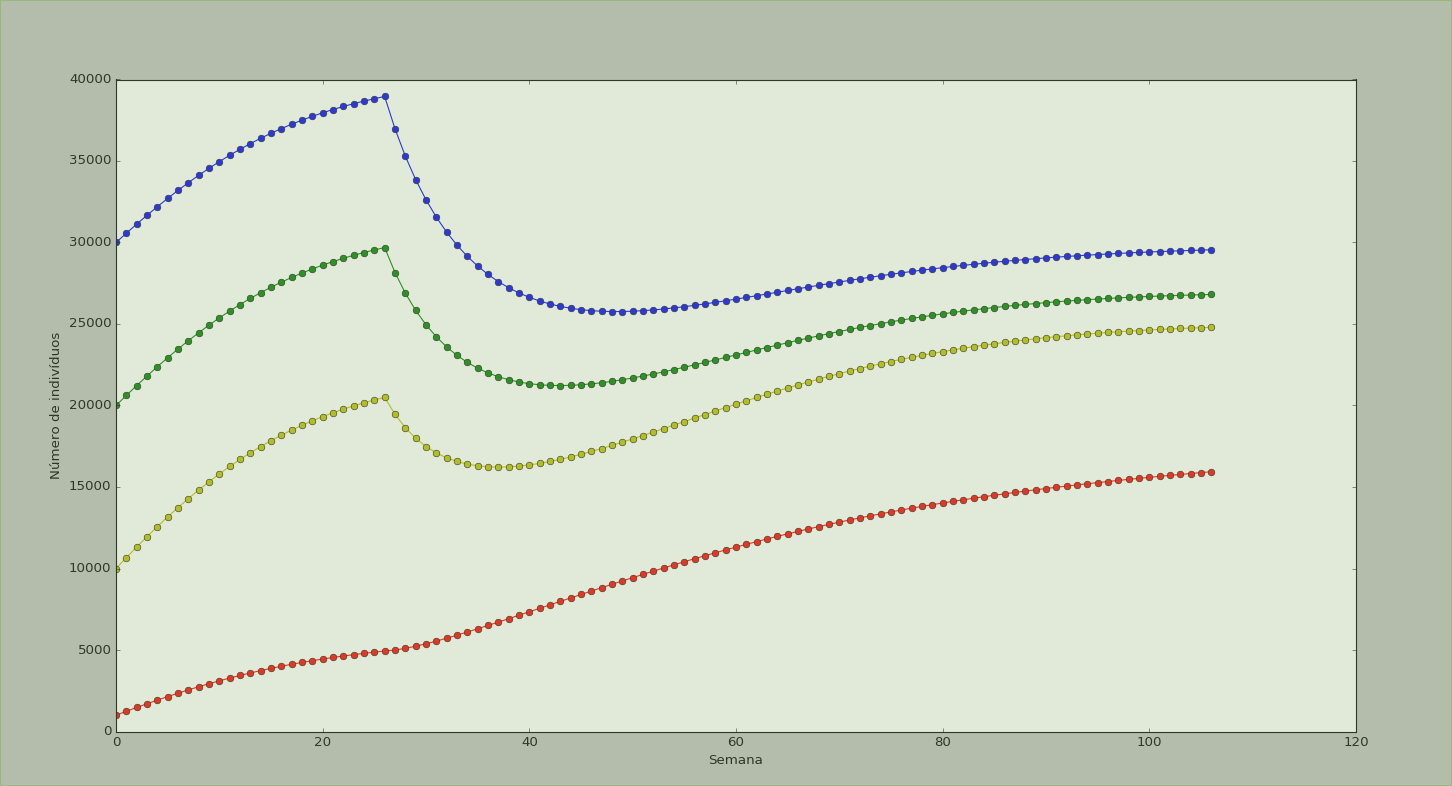
\includegraphics[scale=0.25]{graf_iteracao.png}
\end{figure}
\\
\\
As linhas azul, verde e amarela, representam as presas e a linha vermelha representa o predador.
\\
\\
Analisando os gr\'aficos, podemos ver que a polui\c{c}\~ao influencia muito as presas e faz com seu gr\'afico tenha uma queda brusca. J\'a o predador, por n\~ao ser influenciado pela polui\c{c}\~ao, seu crescimento tamb\'em se altera, por\'em, ao inv\'es de diminuir, ele aumenta.\\
\\
\\
A partir da semana oitenta, podemos ver uma tend\^encia \`a estabilidade do n\'umero de presas. J\'a o n\'umero de predadores continua crescendo e n\~ao vemos a estabilidade do n\'umero de predadores ao longo do per\'iodo de an\'alise.
\\
\\
O gr\'afico abaixo, mostra todas as esp\'ecies e tamb\'em o total de indiv\'iduos (linha preta no gr\'afico).
\\
\\
\begin{figure}[!htb]
\centering
\caption{Gr\'afico da itera\c{c}\~ao entre presa, preadador e polui\c{c}\~ao}
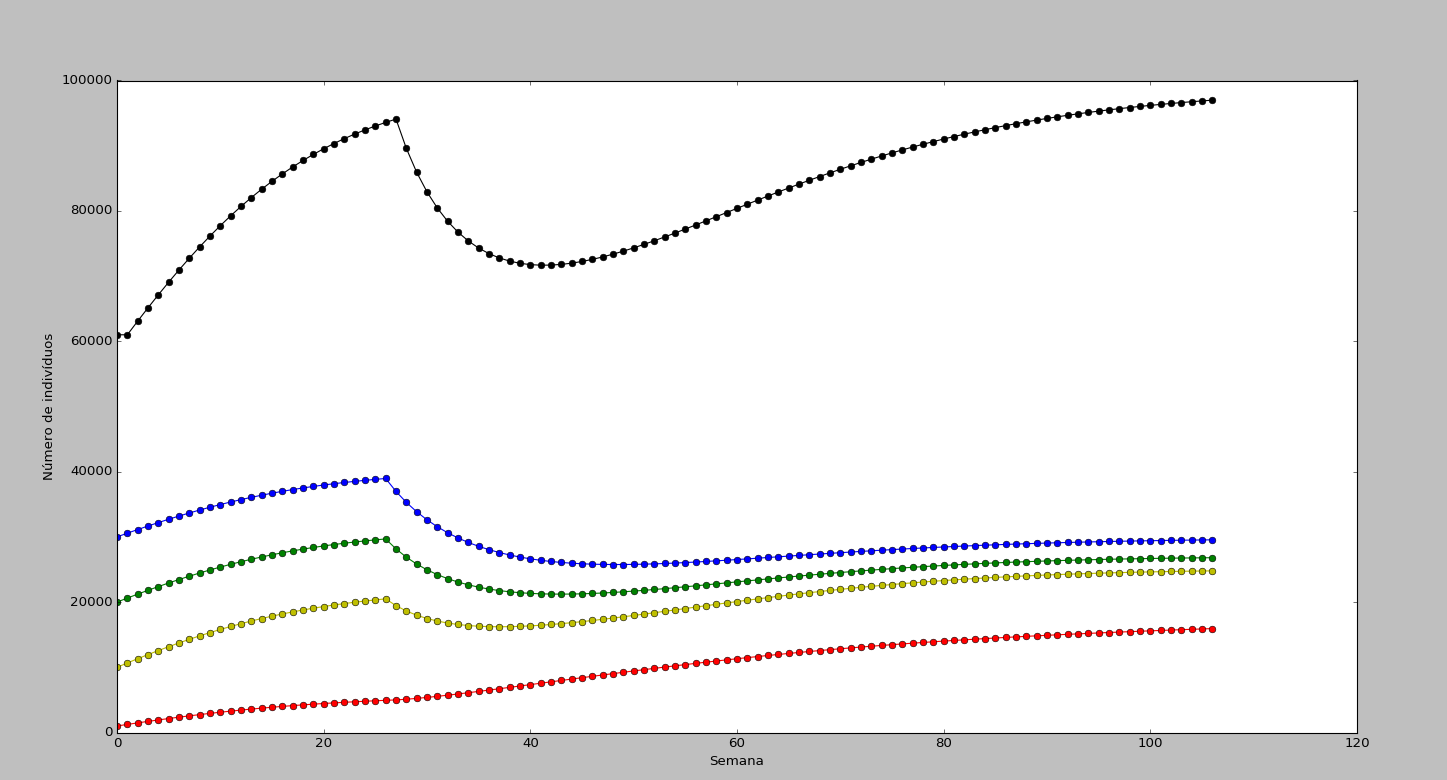
\includegraphics[scale=0.25]{graf_total_ind.png}
\end{figure}
\\
\\
Olhando a popula\c{c}\~ao como um todo, podemos ver a queda brusca no momento em que o poluente \'e introduzido no meio. Vemos, tamb\'em, que existe uma tend\^ecia a instabilidade, que j\'a est\'a sendo alcan\c{c}ada a capacidade de suporte no final das centos e seis semanas.
\\
\\
\'E poss\'ivel que o gr\'afico dos predadores cruze os gr\'aficos de presas ao longo de mais semanas, visto que as presas j\'a est\~ao estabilizando suas popula\c{c}\~oes e o predador ainda continua a crescer.
\\
\\
\section{Conclus\~ao}
O modelo apresentado mostra de forma clara a intera\c{c}\~ao do predador com a presa e tamb\'em o problema do poluente em um meio que era equilibrado. Podemos ver, que para o per\'iodo proposto, o modelo se comporta como o esperado.
\\
\\
Como o predador n\~ao era afetado pela polui\c{c}\~ao, seu crescimento continuou a aumentar mesmo depois da adi\c{c}\~ao do poluente, visto que ainda existia quantidade suficiente de presas para servir de alimento.
\\
\\
O modelo apresentado acima \'e um bom modelo para o per\'iodo analisado, em torno de cem semanas. J\'a para um per\'iodo maior, como por exemplo mil semanas, ele n\~ao se comportar\'a como o esperado, visto que n\~ao foi colocado uma taxa de mortalidade para a popula\c{c}\~ao de predadores. Ent\~ao, ele aumentar\'a muito e se aproximar\'a da capacidade de suporte, extinguindo as presas.
\\
\\
Para um per\'iodo maior de tempo, o modelo precisa ser adaptado incluindo a morte do predador, seja ela por causas naturais, por um outro predador ou pesca.
\end{document}
